\documentclass[a4paper]{article}

%% Language and font encodings
\usepackage[english]{babel}
\usepackage[utf8x]{inputenc}
\usepackage[T1]{fontenc}

%% Sets page size and margins
\usepackage[a4paper,top=3cm,bottom=2cm,left=3cm,right=3cm,marginparwidth=1.75cm]{geometry}

% packages
\usepackage{amsmath, amsfonts}
\usepackage{graphicx, multicol}
\usepackage{textgreek,mathrsfs,bbm,relsize,multirow,float}
\usepackage{amssymb,amsthm,mathtools,scrextend,stackengine}
\usepackage[table,xcdraw]{xcolor} % clashes with tikz package
\usepackage[colorinlistoftodos]{todonotes}
\usepackage{wrapfig}
\newenvironment{frcseries}{\fontfamily{frc}\selectfont}{}
%% commands
\newcommand{\xbar}{\mbox{\larger$\bar{x}$}}
\renewcommand{\baselinestretch}{1.5} %%1.5 spacing
\newcommand{\textfrc}[1]{{\frcseries#1}}
% commands

\newenvironment{sbmatrix}[1]
 {\def\mysubscript{#1}\mathop\bgroup\begin{bmatrix}}
 {\end{bmatrix}\egroup_{\textstyle\mathstrut\mysubscript}}
 
\pgfdeclarelayer{background}
\pgfsetlayers{background,main}

\title{Stats Learning Lecture Week 3}

\begin{document}
\section{Notes}
\textbf{Short videos going over a couple toy data sets in R with each of the key points below}

\subsection{Ensembles}
  An ensemble refers to numerous models being used together to better learn and predict on the same data set. The basic idea behind ensemble learners is that by combining a lot of decent models, they will work together to learn more about the data and create better predictions.
    \subsubsection{Bootstrapping}
    
    Bootstrapping refers to the method of resampling the data with replacement. This is similar to grabbing a handful of marbles out of a bag, placing them back in, and then grabbing another handful from the bag. You could pull out some of the same marbles along with new marbles. 
   
   Below is a diagram form ISLR chapter 5 that gives a nice visual guide to explaining bootstrapping.
   
   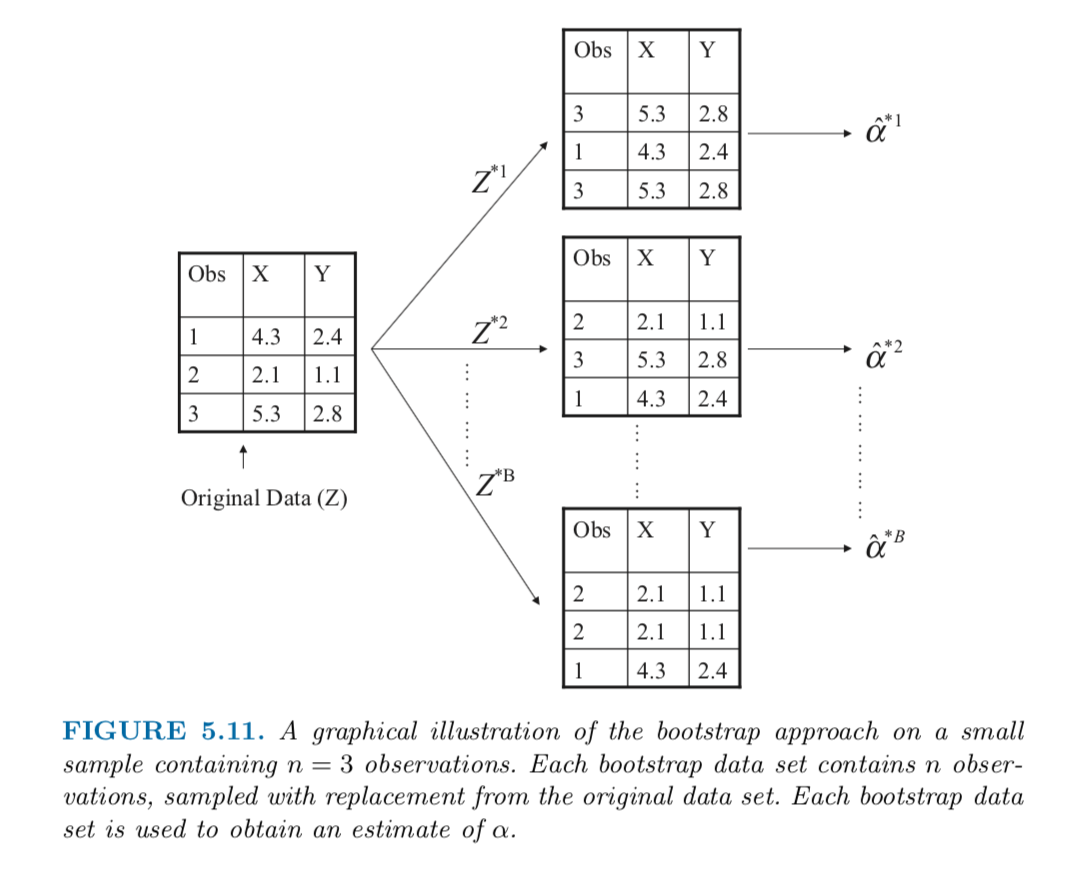
\includegraphics[scale=0.7]{ISLR-boostrap_diagram.png}
   
    \subsubsection{Bagging}
    Bagging is actually just bootstrap aggregating. Bagging is implemented to help reduce the variability of models that may be unstable(like classification trees). However if the model is stable, then bagging has been shown to slightly degrade the performance of the model.
    Lee also states that the $j$th element in a bagged predictor is defined as:
    $$\frac{1}{M}\sum^M_{m=1}G(X,w^{(m)})_j$$
    where $w^{(m)}$ represents the weight of bootstrap $m$ and $G()$ is the function that gives the predictions.

    In general, bagging consists of three basic steps:
    \begin{enumerate}
    \item[1.)] Draw a bootstrap sample from the data  
    \item[2.)] Train a model based on the bootstrap sample and store in the bag of models
    \item[3.)] After created all the models wanted, average the predicted values of all bootstrap models in bag of models on the test set
    \end{enumerate}

    \subsubsection{Random Subspace Learning}
    Random subspace learning is just like bagging, with one exception: instead of using all of the predictors, random subspace learning uses only some. One heuristic to determine the number of predictors used is to round $\sqrt{p}$, where $p$ is the number of predictors, to the nearest integer.

    Similar to bagging, random subspace learning follows a few basic steps:
    In general, bagging consists of three basic steps:
    \begin{enumerate}
    \item[1.)] Randomly select $d\approx\sqrt{p}$ variables to use
    \item[2.)] Draw a bootstrap sample of the $d$ variables from the data  
    \item[3.)] Train a model based on the bootstrap sample and store in the bag of models
    \item[4.)] After created all the models wanted, average the predicted values of all bootstrap models in bag of models on the test set
    \end{enumerate}

  \subsubsection{Boosting}
    Boosting essentially searches and obtains different learners for different portions of the data with each new learner leading to an aggregate performing better than the previous. Adaboost is a version of boosting which is fairly robust to overfitting. Adaboosting's algorithm is as follows:


    \begin{itemize}
    \item Set T, the total number of base learners
    \item Choose a base learner (ie tree or SVM)
    \item Given the data $\mathcal{D}=\{(x_i,y_i),i=1,\dots,n, y\in \{-1,+1\}, x_i\in\mathcal{X}\}$, initialize w at $w^{(1)}=w_1^{(1)},w_2^{(1)},\dots,w_n^{(1)}$ where $w^{(1)}_i=\frac{1}{n}\equiv $weight of observation $i$
    \item For t=1 to T
    \begin{itemize}
    \item train base learner, $h_t$
    \item calculate the error,$\epsilon_t$, of $h_t$ by determining the AUC of $h_t$
    \item determine if $h_t$ passes pre-specified criteria to be a good enough base learner
    \item compute strength of $h_t$; this determines the weight of model $h_t$  $$\alpha_t=\frac{1}{2}log(\frac{1-\epsilon_t}{\epsilon_t})$$
    \item update the weights of all the observations $i=1,\dots,n$
    \begin{itemize}
    \item $\tilde{w}_i^{t+1}=w_i^{(t)}\text{exp}\{-\alpha_ty_ih_t(x_i)\}$
    \item $w_i^{t+1}=$\Large$\frac{\tilde{w}_i^{t+1}}{\sum_{t=1}^T\tilde{w}_i^{t+1}}$
    \end{itemize}
    \end{itemize}
    \end{itemize}

    Thus, $\hat{f}_{boost}(x)=\text{sign}\Big(\sum_{t=1}^T\alpha_th_t(x)\Big)$

\subsection{Model Metrics}
\textbf{\textit{Refer to chapter 6 of ISLR}}

\textbf{\textit{!!! Need to upload something explaining sums of squares (RSS, SST, etc.)}}

The most common metric for determining goodness of fit in a model is MSE, mean squared error. MSE simply find the residuals from the model and the actual data, squares them, and then calculates the mean. Another approach is to then take the square root of the MSE which produces the RMSE, the root mean squared error. Another way of thinking of MSE and RMSE is:

\begin{align*}\text{MSE}=\frac{RSS}{n} && \text{RMSE}=\sqrt{\frac{RSS}{n}} \end{align*}

    While most non statisticians are familiar with the concept of $R^2$, they are most likely not familiar with it's more unbiased cousin $R^2$ adjusted. While still an imperfect measure of goodness of fit, $R^2_{adj}$, is a much better measure for comparing models than $R^2$. Compare them below:
  
  \begin{align*}
  R^2 = 1-\frac{RSS}{SST} && R^2_{adj} = 1-\frac{RSS/(n-p-1)}{SST/(n-1)}=1-\frac{MSE}{MST}
\end{align*}
  
  Notice that $R^2_{adj}$ takes into account the size of the data ($n$ being the number of observations and $p$ being the attributes in the data set). Thus if the model uses more attributes than observations, then it is penalized heavily. Following Occam's razor dictates, $R^2_{adj}$ shows that a simpler model is preferred over an overly complex model.
  
  AIC, Akaike's information criterion, tries to choose the best model by penalizing overly complex models while rewarding models' for how well they fit the data. When comparing models by their AIC, the smaller the AIC the better. Outside of comparing models though, AIC does not say how well a model fits the data.
  
  $$\text{AIC} = 2p+n\text{log}\Big(\frac{RSS}{n}\Big)$$
  
  Similar to AIC, BIC, Bayesian information criterion, is another model metric used for comparing models. Again, when using BIC, the model with the smallest BIC is chosen. Notice that BIC penalizes complex models that rely on few observations more heavily than AIC:
  
  $$\text{BIC} = p\text{log}(n)+n\text{log}\Big(\frac{SSE}{n}\Big)$$

So while AIC tends to choose overly complex models, BIC tends to choose too simple of a model.

Mallow's $C_p$ attempts to bridge the gap between AIC and BIC by penalizing models for using a lot of variables but also rewards models for having a large number of observations. Overall, Mallow's $C_p$ is fairly conservative by over penalizing models to make up for the fact that the model is made with a training set and is likely to be worse when tested on the test set.
  $$\text{Mallows} C_p = \frac{SSE_p}{MSE} +2p-n$$


\subsection{Classification}
Classification refers to data that has a categorical or binary response.

When determining if a classification model properly predicts, a confusion matrix is created. This matrix is a table of the true responses with the predicted responses to see where the model is predicting correctly and where it is predicting incorrectly.

\begin{table}[h]
\centering
\caption{Confusion Matrix}
\label{cm}
\begin{tabular}{l|l|c|c|c}
\multicolumn{2}{c}{}&\multicolumn{2}{c}{Predicted Values}&\\
\cline{3-4}
\multicolumn{2}{c|}{}&Negative&Positive&\multicolumn{1}{c}{}\\
\cline{2-4}
\multirow{2}{*}{True Values}& Negative & $TN$ & $FP$ & $$\\
\cline{2-4}
& Positive & $FN$ & $TP$ & $$\\
\cline{2-4}
\multicolumn{1}{c}{} & \multicolumn{1}{c}{} & \multicolumn{1}{c}{} & \multicolumn{    1}{c}{} & \multicolumn{1}{c}{}\\
\end{tabular}
\end{table}
\begin{align*}
TN&=\text{True Negative, observations that were properly predicted as negative}\\
TP&=\text{True Positive, observations that were properly predicted as positive}\\
FN&=\text{False Negative, observations that were improperly predicted as negative}\\
FP&=\text{False Positive, observations that were improperly predicted as positive}\\
TPR&=\frac{TP}{TP+FN}\equiv\text{True Negative Rate} \\
FPR&=\frac{FP}{FP+TN}\equiv\text{False Positive Rate}
\end{align*}

AUC refers to the Area Under the ROC Curve. The ROC curve is formed by plotting the true positive rate versus the false positive rate (as the y and x values respectively) and is often used to determine how well a model does at prediction compared to random guessing. AUC is the \textbf{a}rea \textbf{u}nderneath this \textbf{c}urve which can be found by calculating the integral of the ROC curve. However, optimizing AUC does not mean that sensitivity and precision will also be optimized. In this case, optimizing sensitivity is a priority so AUC will only be used as an additional metric for comparison between models. AUC determines the probability that the model will rank a minor class instance higher than a major class instance.

%
% AUC GRAPH GOES HERE BUCKOO
%
Also known as recall, sensitivity refers to a model's ability to properly determine when observations are in the minor class.
$$=\frac{TP}{TP+FN}$$

Specificity refers to a models ability to properly determine when observations are part of the major class.
$$=\frac{TN}{TN+FP}$$

The F-measure gives the harmonic mean of sensitivity and precision to show how well the model is doing at accurately predicting the minor class.

\begin{align*}
F-measure&=\frac{2\times \frac{TP}{TP+FN}\times \frac{TP}{TP+FP}}{\frac{TP}{TP+FN}+\frac{TP}{TP+FP}}\\
&=\frac{2\times Sensitivity\times Precision}{Sensitivity+Precision}
\end{align*}

The geometric mean (gmean) gives a geometric average of sensitivity and specificity to show how well the model is doing at predicting both classes overall.
\begin{align*}
G-mean&=\sqrt{\frac{TP}{TP+FN}\times\frac{TN}{TN+FP}}\\
&=\sqrt{Sensitivity\times Specificity}
\end{align*}


\subsection{Cross Validation}
	
    Cross validation is used when creating a model to ensure that a model is created that is accurate without over-fitting. To begin with, a data set will be defined as:
\begin{align*}
\mathcal{D} &= \{(x_i,y_i)\stackrel{\mathclap{\normalfont\mbox{\tiny{iid}}}}{\sim} P_{XY}(x,y),i=1,\dots,n\}\\
&\equiv \text{Given data set}\\
&\equiv \mathcal{L} \cup \mathcal{V} \cup \mathcal{T}\\
&\equiv \mathcal{T}^c\cup\mathcal{T}\\
\mathcal{L}&\equiv\text{Training set}\\ 
&\hspace{16pt}\text{used for learning (fitting) a model}\\
\mathcal{V}&\equiv\text{Validation set}\\ 
&\hspace{16pt}\text{used for tuning hyperparameters withing training set}\\
\mathcal{T}&\equiv\text{Test set}\\ 
&\hspace{16pt}\text{used for proxy to prediction/generalization}
\end{align*}

\begin{wraptable}{r}{7cm}
\caption{Cross Validation visual}\label{CV:1}
\begin{tabular}{lllll}
\multicolumn{5}{l}{$\mathcal{T}^c$}                                                                                                   \\ \hline
\multicolumn{1}{|l|}{$v_1$} & \multicolumn{1}{l|}{$v_2$} & \multicolumn{1}{l|}{$v_3$} & \multicolumn{1}{l|}{$\dots$} & \multicolumn{1}{l|}{$v_m$} \\ \hline
                       &                       &                       &                       &                       \\
                       &                       &                       &                       &                      
\end{tabular}
\begin{tabular}{lllll}
\multicolumn{5}{l}{$\mathcal{T}$}   \\ \hline
\multicolumn{5}{|l|}{} \\ \hline
    &     &    &   &   \\
    &     &    &   &  
\end{tabular}
\newline\begin{tabular}{lllll}
\hline
\multicolumn{1}{|l|}{\cellcolor[HTML]{F8FF00}$v_1$} & \multicolumn{1}{l|}{$v_2$} & \multicolumn{1}{l|}{$v_3$} & \multicolumn{1}{l|}{$\dots$} & \multicolumn{1}{l|}{$v_m$} \\ \hline  
\end{tabular}
\begin{tabular}{|lllll|}
\hline
 &  &  &  &  \\ \hline
\end{tabular}
\newline\begin{tabular}{lllll}
\hline
\multicolumn{1}{|l|}{$v_1$} & \multicolumn{1}{l|}{\cellcolor[HTML]{F8FF00}$v_2$} & \multicolumn{1}{l|}{$v_3$} & \multicolumn{1}{l|}{$\dots$} & \multicolumn{1}{l|}{$v_m$} \\ \hline     
\end{tabular}
\begin{tabular}{|lllll|}
\hline
 &  &  &  &  \\ \hline
\end{tabular}
\newline \begin{tabular}{llllllllll}
 &  &  &  &  &  &  &  &  & \vdots
\end{tabular}
\newline\begin{tabular}{lllll}
\hline
\multicolumn{1}{|l|}{$v_1$} & \multicolumn{1}{l|}{$v_2$} & \multicolumn{1}{l|}{$v_3$} & \multicolumn{1}{l|}{$\dots$} & \multicolumn{1}{l|}{\cellcolor[HTML]{F8FF00}$v_m$} \\ \hline \end{tabular}
\begin{tabular}{|lllll|}
\hline
 &  &  &  &  \\ \hline
\end{tabular}
\end{wraptable} 

You can visualize cross validation as cutting up the data set into your training and test set by making them two separate sections of the data. To start cross validation, you split up the training set into m different chunks. 
 decide on m, the number of chunks you want to split the training set into. This should split it up evenly so that each chunk has the same number of observations. Starting at the first chunk, $v_1$, and continuing to the last chunk,$v_m$, you would disregard one block at a time and train the model with the rest of the chunks in the training set. For each model created, you would then calculate the CV error of each model. The optimal model is then chosen based on the smallest cross validation error. Before going into details, here are some need-to-know  calculations necessary for cross validation.
\bigskip
\newline For $\ell_1,\ell_2,\dots,\ell_{|\mathcal{L}|}\in\mathcal{L}$

\underline{\textbf{Training Error}}\linebreak
$$err(f;\mathcal{L})=\frac{1}{|\mathcal{L}|}\sum_{i=1}^{|\mathcal{L}|}\ell\big(Y_{\ell_{i}},f(x_{\ell_{i}})\big)$$

\underline{\textbf{Validation Error}}\linebreak
$$err(f;\mathcal{V})=\frac{1}{|\mathcal{V}|}\sum_{i=1}^{|\mathcal{V}|}\ell\big(Y_{\textfrc{v}_{i}},f(x_{\textfrc{v}_{i}})\big)$$

\underline{\textbf{Test Error}}\linebreak
$$err(f;\mathcal{T})=\frac{1}{|\mathcal{T}|}\sum_{i=1}^{|\mathcal{T}|}\ell\big(Y_{\textfrc{t}_{i}},f(x_{\textfrc{t}_{i}})\big)$$

Step-By-Step Cross Validation
\newline for (r in 1:m)
\begin{enumerate}
\item leave out rth chunk ($\textfrc{v}_r$)
\item train the function $f$ on $\mathcal{T^c}$ without $\textfrc{v}_r$ and form $\hat{f}(\cdot,\mathcal{T}^c\backslash\textfrc{v}_r,\alpha)\equiv \hat{f}^{(-r)}(\cdot)\equiv \text{estimator built without rth chunk}$
\item $err(\hat{f}^{(-r)},\textfrc{v}_r)=\frac{1}{|\textfrc{v}_r|}\underset{(x_i,y_i)\in\textfrc{v}_r}{\Sigma}\ell(y_i,\hat{f}^{(-r)}(x_i))$
\item $cv(\alpha)=\frac{1}{m}\sum_{r=1}^{m}err(\hat{f}^{(-r)},\textfrc{v}_r,m)$
\end{enumerate}

When you need to tune for hyperparamteters, you would simply put the above loop inside another loop that would run through a sequence for the hyperparameter. You would then choose the setting of the hyperparameter such that
$$\alpha^{opt}\equiv\underset{\alpha\in\text{set}}{\text{argmin}}\{cv(\alpha)\}$$


\section{Homeworks}

\section{AIOs}


\end{document}
